\section{浮点型数据}

\begin{frame}\ft{不同计数法}
\begin{table}
\centering
\begin{tabular}{lll} \hline
数字&科学计数法&指数计数法\\\hline
$1~000~000~000$ & $1.0\times 10^9$ & 1.0e9\\ 
$123~000$ & $1.23\times10^5$ & 1.23e5\\
$322.56$ & $3.2256\times10^2$ & 3.2256e2\\
$0.000~056$ & $5.6\times10^{-5}$ & 5.6e-5\\\hline
\end{tabular}
\end{table}
\end{frame}


\begin{frame}\ft{浮点数的存储方式}
C的浮点数包括\lstinline|float|(单精度)、\lstinline|double|(双精度)和\lstinline|long double|类型。 
\end{frame}
%
%
\begin{frame}\ft{浮点数的存储方式}

C标准规定,
\begin{itemize}
\item \lstinline|float|数据占32位,至少能表示6位有效数字,取值范围至少为$10^{-37}$到$10^{+37}$。
\item \lstinline|double|数据占64位,至少能表示10位有效数字,最小取值范围和\lstinline|float|相同。
\item C只保证\lstinline|long double|类型至少同\lstinline|double|类型一样精确。
\end{itemize}
\vspace{0.1in}

两者在存储方式上都遵从IEEE规范,\lstinline|float|遵从IEEE R32.24,而\lstinline|double|遵从IEEE R64.53。
\end{frame}
%
\begin{frame}\ft{浮点数的存储方式}
无论是单精度还是双精度在存储中都分为三个部分:

\begin{enumerate}
\item
符号位(sign):0代表正,1代表负\\[0.1in]
\item 
指数位(exponent):用于存储科学计数法中的指数数据,并采用移位存储\\[0.1in]
\item 
尾数部分(mantissa)
\end{enumerate}
\end{frame}
% %
\begin{frame}\ft{浮点数的存储方式}
\begin{figure}
\centering
\begin{tikzpicture}
\tikzstyle{bracket} = [decoration={brace,amplitude=1em},decorate,thick,black]
\def\x{0.3}

\draw[fill=blue!20] (0,0)rectangle(-32*\x,2*\x);
\draw (-23*\x,0)--(-23*\x,2*\x);
\draw (-31*\x,0)--(-31*\x,2*\x);
\node at (-11*\x,\x) [] {\footnotesize{23}};
\node at (-27*\x,\x) [] {\footnotesize{8}};
\node at (-31.5*\x,\x) [] {\footnotesize{1}};
%%%% 刻度
\draw (-32*\x,-0.2)--(0*\x,-0.2);
\foreach \i in {0,-1,...,-32}
\draw (\i*\x,-0.2)--(\i*\x,-0.1);
\node at (-0.5*\x,-0.2) [below] {\footnotesize{0}};
\node at (-22.5*\x,-0.2) [below] {\footnotesize{22}};
\node at (-30.5*\x,-0.2) [below] {\footnotesize{30}};

\draw[->,red] (-31.5*\x,-1) node[below]{\footnotesize{符号位}}--(-31.5*\x,-0.2);
\draw[->,red] (-26.5*\x,-1) node[below]{\footnotesize{指数位}}--(-26.5*\x,-0.2);
\draw[->,red] (-12.5*\x,-1) node[below]{\footnotesize{尾数部分}}--(-12.5*\x,-0.2);
\draw [bracket] (-32*\x,2*\x)--node[above=1em]{\footnotesize{32位}}(0*\x,2*\x);


\end{tikzpicture}

\caption{\lstinline|float|数据的存储方式}
\end{figure}
\end{frame}
%
\begin{frame}\ft{浮点数的存储方式}
\begin{figure}
\centering
\begin{tikzpicture}[scale=0.95]
\tikzstyle{bracket} = [decoration={brace,amplitude=1em},decorate,thick,black]
\def\x{0.18}

\draw[fill=blue!20] (0,0)rectangle(-64*\x,2*\x);
\draw (-52*\x,0)--(-52*\x,2*\x);
\draw (-63*\x,0)--(-63*\x,2*\x);
\node at (-26*\x,\x) [] {\footnotesize{52}};
\node at (-57.5*\x,\x) [] {\footnotesize{11}};
\node at (-63.5*\x,\x) [] {\footnotesize{1}};
%%%% 刻度
\draw (-64*\x,-0.2)--(0*\x,-0.2);
\foreach \i in {0,-1,...,-64}
\draw (\i*\x,-0.2)--(\i*\x,-0.1);

\node at (-0.5*\x,-0.2) [below] {\footnotesize{0}};
\node at (-51.5*\x,-0.2) [below] {\footnotesize{51}};
\node at (-62.5*\x,-0.2) [below] {\footnotesize{62}};

\draw[->,red] (-63.5*\x,-1) node[below]{\footnotesize{符号位}}--(-63.5*\x,-0.2);
\draw[->,red] (-57.5*\x,-1) node[below]{\footnotesize{指数位}}--(-57.5*\x,-0.2);
\draw[->,red] (-26.5*\x,-1) node[below]{\footnotesize{尾数部分}}--(-26.5*\x,-0.2);
\draw [bracket] (-64*\x,2*\x)--node[above=1em]{\footnotesize{64位}}(0*\x,2*\x);


\end{tikzpicture}

\caption{\lstinline|double|数据的存储方式}
\end{figure}
\end{frame}
%
\begin{frame}\ft{浮点数的存储方式}
R32.24和R64.53的存储方式都用科学计数法来存储数据。

\begin{li}
120.5的二进制表示为1110110.1,二进制科学计数法表示为1.1101101$\times 2^6$。
\end{li}

\end{frame}
%
\begin{frame}\ft{浮点数的存储方式}
\red{任何一个数的二进制科学计数法表示都为
$$
1.****\times 2^n.
$$
因第一位都是1,不存储,故23位的尾数部分,可表示的精度却是24位。 
} 
\end{frame}
%
\begin{frame}\ft{浮点数的存储方式}
 
\begin{wenti}
那么24位能精确到小数点后几位呢? 
\end{wenti}
因$$
(9)_{10}=(1001)_2,
$$
故四位能精确十进制中的1位小数点,24位就能使\lstinline|float|能精确表示到小数点后6位。
\end{frame}
% %
\begin{frame}\ft{浮点数的存储方式}
关于指数部分,因指数可正可负,8位的指数位能表示的指数范围应该是-127~128。所以指数部分的存储采用移位存储,存储的数据为“原数据+127”。
\end{frame}
%
\begin{frame}\ft{浮点数的存储方式}
以下观察8.25的存储方式: 

\begin{enumerate}
\item $8.25$用二进制的科学计数法表示为$1.0001\times2^3$\\[0.1in] \pause 
\item 符号位为:0,表示为正
\item[] 指数位为:$3+127=130=(1000~0010)_2$
\item[] 尾数部分为:$(0001)_2$\\[0.1in]\pause 
\item 存储方式如下:
\begin{figure}
\centering
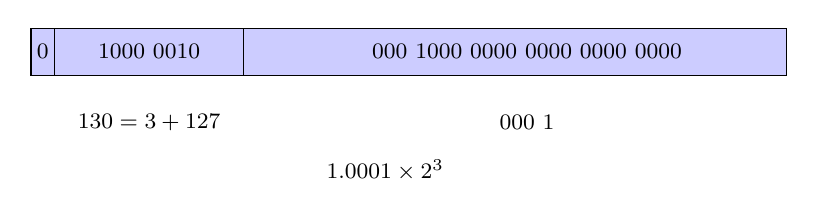
\begin{tikzpicture}
\tikzstyle{bracket} = [decoration={brace,amplitude=1em},decorate,thick,black]
\def\x{0.3}

\draw[fill=blue!20] (0,0)rectangle(-32*\x,2*\x);
\draw (-23*\x,0)--(-23*\x,2*\x);
\draw (-31*\x,0)--(-31*\x,2*\x);
\node at (-11*\x,\x) [] {\footnotesize{000~1000~0000~0000~0000~0000}};
\node at (-27*\x,\x) [] {\footnotesize{1000~0010}};
\node at (-31.5*\x,\x) [] {\footnotesize{0}};

\node at (-27*\x,-2*\x) [] {\footnotesize{$130=\red{3}+127$}};
\node at (-11*\x,-2*\x) [] {\footnotesize{$000~1$}};

\node at (-17*\x,-4*\x) [] {\footnotesize{$1.0001\times 2^3$}};
\end{tikzpicture}
\end{figure}
\end{enumerate}
\end{frame}

\begin{frame}\ft{浮点数的存储方式}
以下观察120.5的存储方式: 

\begin{enumerate}
\item $120.5$用二进制的科学计数法表示为$1.1101101\times2^6$\\[0.1in]\pause 
\item 符号位为:0,表示为正
\item[] 指数位为:$6+127=133=(1000~0101)_2$
\item[] 尾数部分为:$(1101101)_2$\\[0.1in]\pause 
\item 存储方式如下:
\begin{figure}
\centering
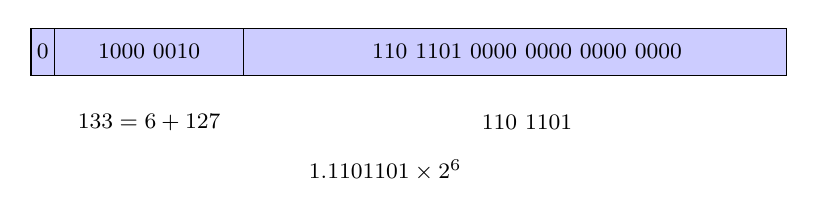
\begin{tikzpicture}
\tikzstyle{bracket} = [decoration={brace,amplitude=1em},decorate,thick,black]
\def\x{0.3}

\draw[fill=blue!20] (0,0)rectangle(-32*\x,2*\x);
\draw (-23*\x,0)--(-23*\x,2*\x);
\draw (-31*\x,0)--(-31*\x,2*\x);
\node at (-11*\x,\x) [] {\footnotesize{110~1101~0000~0000~0000~0000}};
\node at (-27*\x,\x) [] {\footnotesize{1000~0010}};
\node at (-31.5*\x,\x) [] {\footnotesize{0}};

\node at (-27*\x,-2*\x) [] {\footnotesize{$133=\red{6}+127$}};
\node at (-11*\x,-2*\x) [] {\footnotesize{$110~1101$}};

\node at (-17*\x,-4*\x) [] {\footnotesize{$1.1101101\times 2^6$}};
\end{tikzpicture}
\end{figure}
\end{enumerate}
\end{frame}
%
\begin{frame}\ft{浮点数的存储方式}
\begin{wenti}
给出内存中一段数据
$$
0 1000 0101 110 0101 1000 0000 0000 0000,
$$
并告诉你是单精度存储,如何得到该数据的十进制数值?
\end{wenti} 

\end{frame}
%
\begin{frame}\ft{浮点数的存储方式}
\begin{enumerate}
\item 将数据分段
\begin{figure}
\centering
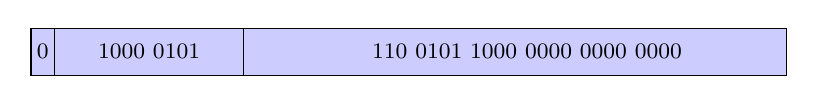
\begin{tikzpicture}
\tikzstyle{bracket} = [decoration={brace,amplitude=1em},decorate,thick,black]
\def\x{0.3}

\draw[fill=blue!20] (0,0)rectangle(-32*\x,2*\x);
\draw (-23*\x,0)--(-23*\x,2*\x);
\draw (-31*\x,0)--(-31*\x,2*\x);
\node at (-11*\x,\x) [] {\footnotesize{110~0101~1000~0000~0000~0000}};
\node at (-27*\x,\x) [] {\footnotesize{1000~0101}};
\node at (-31.5*\x,\x) [] {\footnotesize{0}};
\end{tikzpicture}
\end{figure} \pause 
\item 符号位为0,故为正;因$(1000~0101)_2=133$,故指数为$133-127=6$;故该数据为
$$
(1.1100101\times2^6)_2=(1110010.1)_2=114.5.
$$
\end{enumerate}
\end{frame}
%
\begin{frame}[fragile]\ft{浮点数的存储方式}
阅读如下代码,观察运行结果:
\lstinputlisting[language=c,numbers=left,frame=single]{
ch03/code/float_double.c
}
\end{frame}
%
\begin{frame}[fragile]\ft{浮点数的存储方式}
\begin{lstlisting}
$ gcc float_double.c
$ ./a.out
g1 = 2.2000000476837, g2 = 2.2500000000000
\end{lstlisting}
\end{frame}
%
\begin{frame}[fragile]\ft{浮点数的存储方式}
\begin{wenti}

为什么在单精度转换为双精度时,2.2的数值发生了改变而2.25却没有改变?
\end{wenti} 
\end{frame}
%
\begin{frame}[fragile]\ft{浮点数的存储方式}

\begin{itemize}
\item 2.25的单精度存储方式为
\begin{lstlisting}
0  1000 0001  001 0000 0000 0000 0000
\end{lstlisting}
而双精度存储方式为
\begin{lstlisting}
0  1000 0001  001 0000 0000 0000 0000 0000 0000 0000 0000 0000 0000 0000 0000
\end{lstlisting}
故在强制转换时,数值没有改变。
\end{itemize}

\end{frame}

\begin{frame}[fragile]\ft{浮点数的存储方式}

将十进制小数转换为二进制的方法:\red{将小数乘2,取整数部分。}
\begin{figure}
\centering
\begin{tikzpicture}[scale=0.8]
\matrix[ampersand replacement=\&,matrix of math nodes,column sep=1ex,nodes={inner sep=0.08em}]{
            \& 0 \& .\& 2       \& \&  \\[4pt]
|(a)|\times \&   \&  \&   |(b)|2 \& \&   \\[4pt]
            \& 0 \& .\&  4      \& \& \mbox{取整数位}0 \\[4pt]
|(c)|\times \&   \&  \&  |(d)|2 \& \&   \\[4pt]
            \& 0 \& .\&  8      \& \& \mbox{取整数位}0  \\[4pt]
|(e)|\times \&   \&  \&   |(f)|2 \& \&   \\[4pt]
            \& 1 \& .\&  6      \& \& \mbox{取整数位}1  \\[4pt]                    
|(g)|\times \&   \&  \& |(h)|2 \& \&   \\[4pt]
            \& 1 \& .\& 2      \& \& \mbox{取整数位}1  \\[4pt] 
|(i)|\times \&   \&  \& |(j)|2 \& \&   \\[4pt]
            \& 0 \& .\& 4      \& \& \mbox{取整数位}0  \\[4pt]                                    
};
\draw[thick] (a.south west)--(b.south east)
(c.south west)--(d.south east)
(e.south west)--(f.south east)
(g.south west)--(h.south east)
(i.south west)--(j.south east);
\end{tikzpicture}
\end{figure}
\end{frame}

\begin{frame}[fragile]\ft{浮点数的存储方式}
2.2的二进制表示为一个无限循环的排列:
\begin{lstlisting}
10.0011 0011 0011 0011 0011...
\end{lstlisting}
\end{frame}
%
\begin{frame}[fragile]\ft{浮点数的存储方式}
2.2的单精度存储方式为
\begin{lstlisting}
0  1000 0001  000 1100 1100 1100 1100
\end{lstlisting}
而双精度存储方式为
\begin{lstlisting}
0  1000 0001  000 1100 1100 1100 1100 1100 1100 1100 1100 1100 1100 1100 1100
\end{lstlisting}
故在强制转换时,数值会发生改变。

\end{frame}

\begin{frame}[fragile]\ft{浮点型常量}
基本形式为:
包含小数点的一个带符号的数字序列,接着是字母e或E,然后是代表10的指数的一个有符号值。如
\begin{lstlisting}
-1.56E+12, 2.87e-3
\end{lstlisting}
\end{frame}
%
\begin{frame}[fragile]\ft{浮点型常量}
\begin{itemize}
\item 可以省略正号
\begin{lstlisting}
+2.87e-3
 2.87e-3
\end{lstlisting}
\item 可以没有小数点或指数部分,但不能同时没有
\begin{lstlisting}
2E5
19.28
2     // is an integer
\end{lstlisting}
\item 可以省略小数部分或整数部分,但不能同时省略。
\begin{lstlisting}
3.e12
.45E-5
\end{lstlisting}
\end{itemize}
\end{frame}
%
\begin{frame}[fragile]\ft{浮点型常量}
\begin{itemize}
\item 浮点型常量中不要使用空格
\begin{lstlisting}
1.56 E+12 // wrong
\end{lstlisting}
\item 默认情况下,编译器把浮点型常量当做\lstinline|double|类型。\\[0.1in]
\item[] 设some为一\lstinline|float|变量,
\begin{lstlisting}
some = 4.0 * 2.0;
\end{lstlisting}
则4.0和2.0会被存储为\lstinline|double|类型,用64位存储。
\\[0.1in]
\item[] 注意:乘积运算使用双精度,结果被截取为正常的\lstinline|float|长度,能保证计算精度,但会减慢程序的运行。
\end{itemize}
\end{frame}
%
\begin{frame}[fragile]\ft{浮点型常量}
\begin{itemize}
\item 可以加后缀\lstinline|f|或\lstinline|F|使编译器把浮点常量当做\lstinline|float|型
\begin{lstlisting}
2.3f
3.4e9F
\end{lstlisting}
\item 可以加后缀\lstinline|l|或\lstinline|L|使编译器把浮点常量当做\lstinline|long double|型(由于字母l和数字1容易混淆,建议使用后缀L)
\begin{lstlisting}
54.3l
4.3E9L
\end{lstlisting}
\end{itemize}
\end{frame}

%% add something here
\begin{frame}[fragile]\ft{练习}
\lstinputlisting[language=c,numbers=left,frame=single]{ch03/code/float1.c}
\end{frame}

\begin{frame}[fragile]\ft{练习}
\begin{lstlisting}
$ gcc float1.c
$ ./a.out 
ELSE IF
\end{lstlisting}\pause 


因x为单精度浮点数0.1,常量0.1f表示单精度浮点数0.1,常量0.1f表示双精度浮点数0.1,而根据浮点数的存储方式可知0.1 != 0.1f,故x == 0.1f。
 
\end{frame}



\begin{frame}[fragile]\ft{练习}
\lstinputlisting[language=c,numbers=left,frame=single]{ch03/code/float2.c}
\end{frame}

\begin{frame}[fragile]\ft{练习}
\begin{lstlisting}
$ gcc float2.c
$ ./a.out 
4 8 4
\end{lstlisting}\pause 


原因同上。
\end{frame}


\begin{frame}[fragile]\ft{练习}
\lstinputlisting[language=c,numbers=left,frame=single]{ch03/code/float3.c}
\end{frame}

\begin{frame}[fragile]\ft{练习}
\begin{lstlisting}
$ gcc float2.c
$ ./a.out 
IF
\end{lstlisting}\pause 


因x为单精度浮点数0.5,常量0.1f表示单精度浮点数0.5,常量0.5f表示双精度浮点数0.5,但是根据浮点数的存储方式可知0.5 == 0.5f,故条件x == 0.5先满足,从而执行第一个分支。

\end{frame}

% %
\begin{frame}[fragile]\ft{打印浮点型数据}
\begin{itemize}
\item 使用格式说明符\lstinline|%f|打印\lstinline|float|和\lstinline|double|型数据,{\tf \%e}打印指数计数法的数字。\\[0.1in]
\item 使用格式说明符\lstinline|%Lf|、{\tf \%Le}打印\lstinline|long double|型数据。
\end{itemize}
\end{frame}

\begin{frame}[fragile]\ft{打印浮点型数据}
\lstinputlisting[language=c,numbers=left,frame=single]{ch03/code/showf_pt.c}
\end{frame}

\begin{frame}[fragile]\ft{打印浮点型数据} 
\begin{lstlisting}
$ gcc showf_pt.c
$ ./a.out
32000.000000 can be written as 3.200000e+04
2140000000.000000 can be written as 2.140000e+09
0.000053 can be written as 5.320000e-05
\end{lstlisting}
\end{frame}
%
\begin{frame}[fragile]\ft{浮点型数据的上溢和下溢}
\lstinputlisting[language=c,numbers=left,frame=single]{ch03/code/float_overflow.c}
\end{frame}
%
\begin{frame}[fragile]\ft{浮点型数据的上溢和下溢}\begin{lstlisting}
$ gcc float_overflow.c
$ ./a.out
toobig = inf
\end{lstlisting}

\end{frame}
%
\begin{frame}[fragile]\ft{浮点型数据的上溢和下溢}
当浮点数超出表示范围时,会发生上溢(overflow),C会赋予一个代表无穷大的特殊值,即inf。

\end{frame}
%
\begin{frame}[fragile]\ft{浮点型数据舍入误差}
\lstinputlisting[language=c,numbers=left,frame=single]{ch03/code/float_err.c}
\end{frame}
%
\begin{frame}[fragile]\ft{浮点型数据舍入误差}
\begin{lstlisting}
$ gcc float_err.c
$ ./a.out
b = 4008175468544.000000
\end{lstlisting}
\end{frame}
%
\begin{frame}[fragile]\ft{浮点型数据舍入误差}
为什么会出现如此奇怪的结果?原因是计算机缺乏足够的进行正确运算所需的十进制位数。
\vspace{0.1in}

数字2.0e20加1,变化的是第21位,要计算正确,至少需要存储21位的数字,而\lstinline|float|型数字只有6、7位有效数字,故该计算注定不正确。
\end{frame}
%
% %
% %
